\documentclass{article}

\usepackage{amssymb}
\usepackage{mathtools}
\usepackage{amsmath}
\usepackage{amsthm}
\usepackage{babel}
\usepackage{stackengine}
\usepackage{tikz}
\usepackage{tikz-cd}
\usepackage{quiver}
\usepackage{mathrsfs}
\usepackage{braket}
\usepackage{float}
\usepackage{scalerel}
\usepackage{stackengine,wasysym}
\usepackage{blindtext}
\usepackage[final]{hyperref}
\usepackage{bbold}
\usepackage{geometry}
\usepackage{cancel}
\usepackage{booktabs}
\usepackage{comment}

\title{Investigating RR--NS Interactions Using Measurement Structures}
\author{Ryan J. Buchanan\footnote{Active Inference Institute, Cascadia, USA. ORCiD: \href{https://orcid.org/0009-0000-1253-0031}{0009-0000-1253-0031} }}
\date{June, 2026}

\newtheorem{war}{Warning}
\newtheorem{dn}{Definition}
\newtheorem{as}{Assumption}
\newtheorem{rk}{Remark}
\newtheorem{eg}{Example}
\newtheorem{pp}{Proposition}
\newtheorem{ax}{Axiom}
\newtheorem{tm}{Theorem}
\newtheorem{lem}{Lemma}
\newtheorem{nt}{Notation}
\newtheorem{prop}{Property}
\newtheorem{rc}{Recollection}
\newtheorem{exc}{Exercise}
\newtheorem{setup}{Setup}

\numberwithin{tm}{section}
\numberwithin{dn}{section}
\numberwithin{as}{section}
\numberwithin{rk}{section}
\numberwithin{lem}{section}
\numberwithin{ax}{section}
\numberwithin{pp}{section}
\numberwithin{eg}{section}
\numberwithin{war}{section}
\numberwithin{equation}{section}
\numberwithin{prop}{section}
\numberwithin{nt}{section}
\numberwithin{rc}{section}
\numberwithin{setup}{section}

\newcommand\restr[2]{{%
		\left.\kern-\nulldelimiterspace
		#1
		\right|_{#2}
}}

\def\code#1{\texttt{#1}}

\begin{document}
	\maketitle

\begin{abstract}
	This paper develops heuristic framework for Ramond--Ramond (RR) and Neveu--Schwarz (NS) interactions by combining the convexity monad with geometric models of string and brane dynamics. We work with \emph{measurement structures} (defined here), in which generalized states are encoded as elements of the monad and observables arise as pushforwards along Hamiltonians. We describe local RR charges and NS backgrounds in terms of integrals of an RR one-form over windows and orbits, mimicking Wess--Zumino and Chern--Simons-type couplings in a purely convex setting. This viewpoint makes precise how RR flux profiles on circles, tori, and nontrivial fibrations induce local couplings $\kappa$ that control string--brane and string--string interaction amplitudes, and the Gregory--Harvey--Moore (GHM) unwinding mechanism is replicated. As an application, we show that the radion sector of two-brane Randall--Sundrum models can be incorporated into the same formalism by treating brane tensions and radion configurations as additional observables, and we construct an effective coupling $\kappa_{\mathrm{RS}}$ as a convex functional of the induced distribution of tension traces, engineered to mirror the inverse-VEV and instability structure of RR--NS couplings. The result is a monadic framework in which local couplings, charge inflow, and radion-like degrees of freedom all arise from a common convex, monadic description of measurement.
\end{abstract}

\pagebreak

\tableofcontents
	
	\section{Convexity Monad} \label{Convexity}
	
	Let us recall the following definition from \cite{Haderi}:
	
	\begin{dn} 
		Let $\mathbf{R}$ be a semiring. The \emph{convexity monad} is the functor
		\begin{align} \label{mono1}
			D_R: \mathrm{Set} \longrightarrow \mathrm{Set},
			\qquad
			D_R(X) \coloneq \left\{ p: X \to R \;\middle|\; p \text{ is finitely supported, } \sum_{x \in X} p(x) = 1 \right\}.
		\end{align}
	\end{dn}
	
	Because of its resemblance to classical probability distributions, this is often referred to as the \emph{distribution monad}. Given a function $f: X \to M$, there is an induced pushforward map
	\begin{align}
		f_* : D_R(X) \longrightarrow D_R(M),
	\end{align}
	defined by
	\begin{align}
		f_*(p)(\mu) = \sum_{x \in f^{-1}(\mu)} p(x).
	\end{align}
	
	This construction allows us to interpret elements of $D_R(X)$ as generalized states, and the pushforward as the propagation of such states along observables.
	
	Now let $X$ be a state space and let
	\begin{align}
		H: X \longrightarrow \mathbb{R}
	\end{align}
	be a Hamiltonian. Denote by
	\begin{align}
		\Gamma \coloneq H(X) \subseteq \mathbb{R}
	\end{align}
	the space of attainable energy values. Then any distribution $p \in D_R(X)$ induces a distribution on $\mathbb{R}$ via
	\begin{align}
		H_* : D_R(X) \longrightarrow D_R(\mathbb{R}),
	\end{align}
	given explicitly by
	\begin{align}
		H_*(p)(\gamma) = \sum_{x \in H^{-1}(\gamma)} p(x).
	\end{align}
	
	In this way, the convexity monad encodes the passage from states to measurement outcomes. Reality constraints \cite{Smooth} suggest restricting to the case $R = \mathbb{R}$, so that $D_R(X)$ may be interpreted as a space of probabilistic states.
	
\section{Measurement Structures and RR Charges}

The construction above may be viewed as monocolored, in the sense that the convex structure is applied to a single type of object. We now extend this perspective to incorporate a simple internal symmetry, with an eye towards charge-like observables.

\begin{dn} \label{measurement structure}
	The \emph{measurement structure} is a two-colored\footnote{This terminology is informal. For genuine colored operads, see Yau \cite{Yau}.} structure consisting of:
	\begin{enumerate}
		\item A state space $X$ together with a Hamiltonian $H: X \to \mathbb{R}$,
		\item A $U(1)$-equivariant fiber bundle $\pi: X \to Y$, where $Y$ is a smooth manifold,
	\end{enumerate}
	together with the assignment
	\begin{align}
		(p,H,\pi) \longmapsto H_*(p) \in D_{\mathbb{R}}(\mathbb{R}),
	\end{align}
	where $p \in D_{\mathbb{R}}(X)$.
\end{dn}

Here the group $U(1)$ is understood as the internal symmetry of phase rotations. This choice is physically natural, since it is the standard symmetry associated with conserved charge and provides a convenient model for charge-like measurement data. In particular, it offers a simple setting in which one may later consider more elaborate notions of charge, including those appearing in string-theoretic contexts.

The role of the bundle $\pi: X \to Y$ is to encode geometric or background data, while the Hamiltonian mediates the passage from states to observable values. The $U(1)$-equivariance ensures that the measurement procedure is compatible with the internal symmetry, so that the resulting distribution depends only on the symmetry-respecting structure of the system.

\begin{eg}
	As a simple illustration, let $X=\mathbb{R}^2$ and let $G=U(1)$ act on $X$ by rotations. Equivalently, for $\theta \in \mathbb{R}$ we write
	\[
	R(\theta)=
	\begin{pmatrix}
		\cos\theta & -\sin\theta\\
		\sin\theta & \cos\theta
	\end{pmatrix},
	\]
	so that $R(\theta)\cdot x$ is the rotated vector.
	
	Now let
	\[
	H:X\to \mathbb{R}, \qquad H(x)=\|x\|^2
	\]
	be a $U(1)$-invariant Hamiltonian. Indeed,
	\[
	H(R(\theta)x)=\|R(\theta)x\|^2=\|x\|^2=H(x)
	\]
	for all $\theta$.
	
	Consider the finitely supported distribution
	\[
	p=\tfrac12\delta_{e_1}+\tfrac12\delta_{e_2}
	\]
	in $D_{\mathbb{R}}(X)$, where $e_1=(1,0)$ and $e_2=(0,1)$. Since
	\[
	H(e_1)=H(e_2)=1,
	\]
	the pushforward distribution along $H$ is concentrated at the single value $1$:
	\[
	H_*(p)=\delta_1.
	\]
	
	Thus the measurement procedure forgets the particular phase representative of the state and records only the symmetry-invariant observable value. In this elementary case, the $U(1)$-equivariance is exactly what makes the measurement compatible with the internal symmetry.
\end{eg}

\begin{dn}
	Let $G$ be a group acting on a set $X$. An observable
	\[
	H : X \to \mathbb{R}
	\]
	is called \emph{$G$-admissible} if it is $G$-invariant, i.e.
	\[
	H(g\cdot x) = H(x)
	\]
	for all $g \in G$ and $x \in X$.
\end{dn}

\begin{rk}
	We record some examples of admissible measurements in the context of type-0 string theories in the appendix \S\ref{two}.
\end{rk}

\begin{pp} \label{pp}
	Let $G$ act on $X$, and let $H : X \to \mathbb{R}$ be a $G$-admissible observable. Suppose $p \in D_{\mathbb{R}}(X)$ is a distribution which is $G$-invariant in the sense that
	\[
	p(g\cdot x) = p(x)
	\]
	for all $g \in G$ and $x \in X$. Then the pushforward distribution
	\[
	H_* (p) \in D_{\mathbb{R}}(\mathbb{R})
	\]
	depends only on the $G$-orbits in $X$. In particular, $H_*(p)$ is invariant under any transformation of $X$ induced by the $G$-action.
\end{pp}

\begin{proof}
	By definition,
	\[
	H_*(p)(\gamma) = \sum_{x \in H^{-1}(\gamma)} p(x).
	\]
	Since $H$ is $G$-invariant, each fiber $H^{-1}(\gamma)$ is a union of $G$-orbits. Moreover, $p$ is constant on each orbit by $G$-invariance. Thus the value $H_*(p)(\gamma)$ is determined entirely by how much total weight $p$ assigns to the union of orbits contained in $H^{-1}(\gamma)$, and this does not change if we replace $p$ by any distribution obtained by redistributing mass within individual $G$-orbits. Hence $H_*(p)$ depends only on the orbit structure, and is insensitive to the choice of representatives within each orbit.
\end{proof}

\section{Generative RR--NS Dynamics} \label{RRNS}

In Appendix~\S\ref{two}, a more general case is considered, where a system factorized into two $U(1)$ sectors can collapse into just one. When this happens, we have a distinguished orbit $\mathfrak{o}$ whose admissible dynamics are frozen. However, we may equally well consider a more complicated system in which there happens to be a third $U(1)$ sector. Our treatment of RR and NS charges in terms of integrals of $C_{(1)}$ and $B_{(2)}$ fits naturally into the broader picture of D-brane charges and Ramond--Ramond fields developed in the late 1990s. In particular, it is compatible with the viewpoint that RR charges are measured by integrals of RR fluxes over cycles and are classified by (generalized) cohomological invariants, as in the K-theoretic descriptions of Minasian--Moore \cite{MinasianMoore} and Witten \cite{WittenKtheory}, while our use of these integrals to define a local, convexity-compatible coupling is novel in that it ties these structures directly to a measurement-theoretic framework rather than to global charge quantization.

\medskip

 Instead of collapsing a circle to a point, we can then collapse a \emph{torus} to a \emph{pair of points}:
\[
T^2 \longrightarrow \mathfrak{o}_1 \cup \mathfrak{o}_2
\]
and form a window $\mathfrak{O} \coloneq [\mathfrak{o}_1, \mathfrak{o}_2]$ such that this union is equal to $\partial \mathfrak{O}$.

If the stabilizer of $\mathfrak{O}$ in $G$,
\[
\mathrm{Stab}_G(\mathfrak{O}) \coloneq \{\, g \in G \mid g \cdot \mathfrak{O} = \mathfrak{O} \,\},
\]
is a subgroup of $G$, then this subgroup will be admissible. When this is the case, the KK-compactification has non-trivial dynamics, and is thus $G$-admissible but not KK-admissible. In particular, for all $g \in \mathrm{Stab}_G(\mathfrak{O})$ and all $x \in X$ we have
\[
p(g \cdot x) = p(x) .
\]
Our fiber bundle $\pi$ in Definition~\ref{measurement structure} then restricts to a bundle
\[
\pi|_{\mathfrak{O}} : \mathfrak{O} \longrightarrow Y_0
\]
for some submanifold $Y_0 \subseteq Y$. Taking sections $\pi^{-1}(\{y\})$ of sequences $\{y\} \in Y_0$ yields a sub-window $\mathcal{B}_1$ of the non-trivial toroidal sector of the RR field.

\subsection{String--Brane Interactions}\label{SB}
Let us suppose $\mathcal{B}_1$ is a brane of dimension $1$. Then integrating the Hamiltonian along $\mathcal{B}_1$,
\begin{equation}
	C_{(1)} \coloneq \int_{\mathcal{B}_1} H(x) = \int_X \Omega,
\end{equation}
is equivalent to integrating a $1$-form $\Omega$ over $X$, which we interpret as a Ramond--Ramond charge.\footnote{The $1$-form is induced by the restriction of the Hamiltonian density to the brane sector.} To obtain a corresponding Neveu--Schwarz (NS) charge associated with the endpoint of a string coupled to an external brane $\mathcal{B}_3$, we define a two-form
\begin{equation}
	B_{(2)} \coloneq d C_{(1)} \wedge \mathrm{Tr}\, C_{(1)} .
\end{equation}
where we regard $\mathrm{Tr} \; C_{(1)}$ as a scalar-valued density obtained from the local RR profile.

Notice that the result is only a two-form; this is because the mass of the string is constrained to lie on an invariant subspace of $\mathfrak{O}$.

In our approach, we will let
\[
\kappa \coloneq \int \mathrm{Tr}\, C_{(1)}
\]
be the \emph{RR-NS coupling}. The integral is not yet specified globally; in practice we bound it by a subwindow of $\mathfrak{O}$. If $\kappa$ is to remain physical, it must lie in the semifield $\mathbb{R}_{\geq 0}$, as studied in~\cite{Haderi}.

\begin{rk}
	We emphasize that $\kappa$ is not intended as a fundamental string coupling derived from perturbative string theory, but rather as an effective local functional within the framework introduced here.

	One may view $\kappa = \int \mathrm{Tr}\, C_{(1)}$ as a local analogue of the way RR charges and fluxes are traditionally captured by integrals of RR field strengths over cycles, as in the K-theoretic classification of D-brane charge. The novelty here is that the same integral is used to produce an effective coupling compatible with the convexity structure of $D_{\mathbb{R}}(X)$, rather than a global topological charge class.
\end{rk}

\begin{figure}[H]
	\centering
	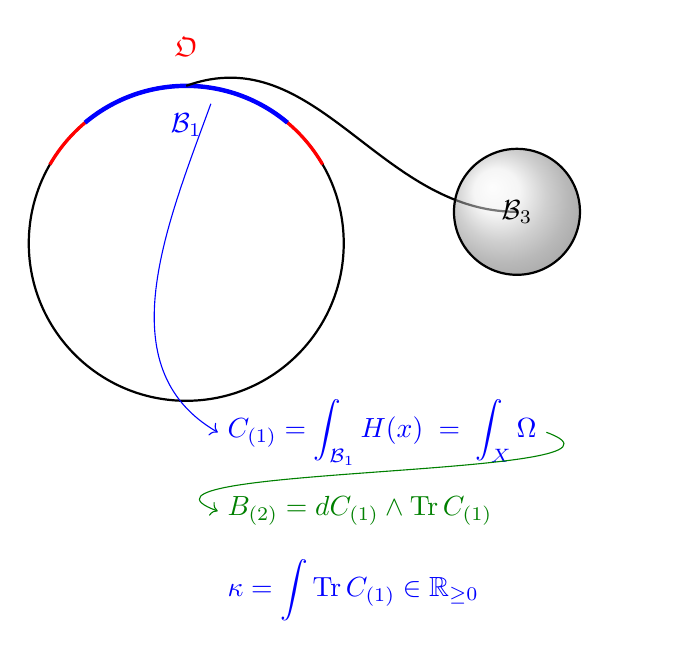
\begin{tikzpicture}[scale=2]
		
		% Circle
		\draw[thick] (0,0) circle (1);
		
		% Red arc O (from 30 to 150 degrees, say)
		\draw[very thick,red] (30:1) arc (30:150:1);
		\node[red] at (90:1.25) {$\mathfrak{O}$};
		
		% B1 as a segment along the circle inside O
		\draw[ultra thick,blue] (50:1) arc (50:130:1);
		\node[blue] at (90:0.75) {$\mathcal{B}_1$};
		
		% String from a point on O to the 3-brane – curved so it avoids the circle
		\coordinate (attach) at (90:1); % point on the circle
		\coordinate (braneCenter) at (2.1,0.2);
		\draw[thick]
		(attach) to[out=20,in=180] (braneCenter);
		
		% 3d brane B3 as a shaded disk
		\shade[ball color=gray!20,opacity=0.5] (braneCenter) circle (0.4);
		\draw[thick] (braneCenter) circle (0.4);
		\node at (2.1,0.2) {$\mathcal{B}_3$};
		
		% Equation C_{(1)} with curved arrow from B1
		\node[blue,right] (Ceq) at (0.2,-1.2)
		{$C_{(1)} = {\displaystyle\int_{\mathcal{B}_1} H(x)} \;=\; {\displaystyle\int_X \Omega}$};
		\draw[->,blue]
		(80:0.9) to[out=-110,in=150] (Ceq.west);
		
		% Equation B_{(2)} with curved arrow from C_{(1)}
		\node[green!50!black,right] (Beq) at (0.2,-1.7)
		{$B_{(2)} = d C_{(1)} \wedge \mathrm{Tr}\, C_{(1)}$};
		\draw[->,green!50!black]
		(Ceq.east) to[out=-20,in=160] (Beq.west);
		
		% Equation kappa with curved arrow from C_{(1)}
		\node[blue,right] (keq) at (0.2,-2.2)
		{$\kappa = {\displaystyle\int \mathrm{Tr}\, C_{(1)}} \in \mathbb{R}_{\ge 0}$};
		
	\end{tikzpicture}
	\caption{Local measurement structure for RR and NS charges: a window $\mathfrak{O}$ on a circle, a 1-brane $\mathcal{B}_1$ along the window, and a string ending on a 3-brane $\mathcal{B}_3$. The integrals define $C_{(1)}$, the NS two-form $B_{(2)}$, and the local coupling $\kappa \in \mathbb{R}_{\ge 0}$.}
	\label{fig:local_rr_ns_measurement}
\end{figure}

\begin{rk}
	The definition of $C_{(1)}$ and the derived two-form $B_{(2)}$ is inspired by the familiar Wess--Zumino and Chern--Simons couplings \cite{Alekseev} of RR potentials to D-brane worldvolume gauge fields, where wedge products of RR forms with traces of gauge field strengths encode induced lower-dimensional charges. In our setting, the role of the worldvolume gauge field is played by the Hamiltonian $H$ integrated along the brane $\mathcal{B}_1$, and the combination $dC_{(1)} \wedge \mathrm{Tr}\,C_{(1)}$ should be thought of as a toy model for such induced NS--NS couplings, expressed directly in the language of measurement structures.
\end{rk}

\subsection{String--String Interactions} \label{SS}
We now consider a second external brane $\mathcal{B}'_3$, and strings with one endpoint on $\mathcal{B}_3$ and the other on $\mathcal{B}'_3$. Let $\Sigma$ denote the worldsheet of such an open string, with boundary
\[
\partial \Sigma = \gamma_3 \cup \gamma'_3,
\]
where $\gamma_3 \subset \mathcal{B}_3$ and $\gamma'_3 \subset \mathcal{B}'_3$ are the respective boundary segments.

\begin{dn}
	Given a local coupling $\kappa = \displaystyle\int \mathrm{Tr}\, C_{(1)} \in \mathbb{R}_{\ge 0}$, the \emph{interaction amplitude} for an open string with one endpoint on $\mathcal{B}_3$ and the other on $\mathcal{B}'_3$ is weighted by
	\[
	\mathcal{A}_{\mathrm{int}}(\Sigma) \;\propto\; \exp\!\left( - \kappa \int_{\Sigma} B_{(2)} \right),
	\]
	where $B_{(2)} = d C_{(1)} \wedge \mathrm{Tr}\, C_{(1)}$ is the NS two-form defined above.
\end{dn}

\begin{rk}
	In this formulation, $\kappa$ controls the strength with which strings ending on $\mathcal{B}_3$ and $\mathcal{B}'_3$ couple to the NS background $B_{(2)}$. Increasing $\kappa$ enhances the effective interaction strength between the two branes mediated by such strings, while decreasing $\kappa$ suppresses it. Since $\kappa$ itself is defined by integrating $\mathrm{Tr}\,C_{(1)}$ over the RR window $\mathfrak{O}$, the inter-brane coupling is directly determined by the local RR configuration captured by the measurement structure.
\end{rk}

Informally, one expects the interaction amplitude to increase as the window $\mathfrak{O}$ shrinks. The intuition is that, for a fixed total RR content, concentrating the support of $\mathrm{Tr}\,C_{(1)}$ into a smaller region of the circle forces its local density to grow, so that the integral defining $\kappa$ becomes larger when evaluated along $\mathfrak{O}$. Since the inter-brane amplitude is weighted by $\exp(-\kappa \int_{\Sigma} B_{(2)})$, this enhancement of $\kappa$ strengthens the effective coupling between strings ending on $\mathcal{B}_3$ and $\mathcal{B}'_3$.

A loose way to see this is as follows. Fix a non-negative profile for $\mathrm{Tr}\,C_{(1)}$ on the circle, and suppose it is initially spread over a larger arc containing $\mathfrak{O}$. If we now shrink the window $\mathfrak{O}$ while keeping the total integrated RR content over the larger arc approximately fixed, the restriction of $\mathrm{Tr}\,C_{(1)}$ to the smaller $\mathfrak{O}$ must increase in magnitude on average. In other words, the same amount of RR ``charge'' is forced through a smaller angular region. Since $\kappa$ is obtained by integrating $\mathrm{Tr}\,C_{(1)}$ along $\mathfrak{O}$, this concentration effect increases $\kappa$ as the window shrinks. Consequently, the exponential weight in the interaction amplitude becomes larger in magnitude, reflecting a stronger effective coupling between the two branes mediated by strings whose endpoints lie inside the more sharply localized window. 

Given the standard coupling \cite{Tseytlin}
\begin{equation}
	S_B[\Sigma] = \int_{\Sigma} B_{(2)}
\end{equation}
the effective coupling between the strings is then:
\begin{equation}
	g_{\mathrm{eff}} (\mathfrak{O}) = \kappa (\mathfrak{O}) \int_\Sigma B_{(2)} (\mathfrak{O}).
\end{equation}

\section{Winding Charge Inflow and the Boundary Orbits} \label{winding}

In \S\ref*{SS} we observed that as the window $\mathfrak{O}$ shrinks, the coupling $\kappa$ grows and the interaction amplitude $\mathcal{A}_{\mathrm{int}}(\Sigma)$ is enhanced. We now give a dynamical explanation for \emph{why} charge accumulates at the boundary orbits $\mathfrak{o}_1, \mathfrak{o}_2 = \partial\mathfrak{O}$, by showing that the topology of $\mathfrak{O}$ forces winding charge to flow there whenever a wound string unwinds inside the window. The argument is a measurement-theoretic adaptation of the unwinding mechanism of Gregory--Harvey--Moore (GHM) \cite{GHM}.

\subsection{Nontrivial Fibration over the Window}

Recall from \S\ref{RRNS} that the restricted bundle $\pi|_{\mathfrak{O}} : \mathfrak{O} \to Y_0$ has fibers which are orbits of the stabilizer $\mathrm{Stab}_G(\mathfrak{O})$. We now impose the following topological assumption.

\begin{as} \label{hopf-as}
	The total space of $\pi|_{\mathfrak{O}} : \mathfrak{O} \to Y_0$ is a nontrivial $S^1$ fibration over $Y_0 \cong S^2$, so that $\mathfrak{O}$ is topologically $S^3$. In particular, $\pi_1(\mathfrak{O}) = 0$.
\end{as}

This is precisely the topology of the Hopf fibration, which is the global structure at spatial infinity in the Kaluza-Klein monopole background. The key consequence is that although the $S^1$ fiber appears nontrivial locally (a string wound once around a fiber at a generic point of $Y_0$ cannot be contracted within that fiber) it \emph{is} contractible globally within $\mathfrak{O}$, since $\pi_1(S^3) = 0$.

\subsection{Unwinding and Charge Conservation}

Let $\mathcal{B}_1 \subset \mathfrak{O}$ be the 1-brane of \ref{RRNS}, understood now as a string wound once around the $S^1$ fiber of $\pi|_{\mathfrak{O}}$ at a point $y_0 \in Y_0$. Since $\pi_1(\mathfrak{O}) = 0$ by Assumption~\ref{hopf-as}, this string can be unwound by a continuous motion within $\mathfrak{O}$ while remaining arbitrarily far from the boundary $\partial\mathfrak{O}$.

However, the winding number of a string around the fiber is a conserved charge---it couples to the RR one-form $C_{(1)}$ defined in \S\ref{SB}. More precisely, the integral
\[
\mathcal{W}(\mathcal{B}_1) \coloneq \oint_{\mathcal{B}_1} C_{(1)}
\]
is the H-electric winding charge of the string, and it is conserved by the equation of motion derived from the standard coupling $S_B[\Sigma] = \int_\Sigma B_{(2)}$. Since the winding of $\mathcal{B}_1$ changes from $1$ to $0$ during the unwinding motion, this charge cannot simply disappear. By the same inflow argument as in \cite{GHM}, it must be transferred to a localized source. The only available sources in our setup are the boundary orbits $\mathfrak{o}_1$ and $\mathfrak{o}_2 = \partial\mathfrak{O}$.

\begin{pp} \label{inflow}
	Under Assumption~\ref{hopf-as}, whenever the wound string $\mathcal{B}_1$ unwinds within $\mathfrak{O}$, the winding charge $\mathcal{W}(\mathcal{B}_1)$ flows to the boundary $\partial\mathfrak{O} = \mathfrak{o}_1 \cup \mathfrak{o}_2$.
\end{pp}

\begin{proof}
	Since $\pi_1(\mathfrak{O})=0$, there exists a homotopy $\{b_t\}_{t\in[0,1]}$ of loops within $\mathfrak{O}$ with $b_0 = \mathcal{B}_1$ (wound) and $b_1$ contractible. The charge $\mathcal{W}(b_t) = \oint_{b_t} C_{(1)}$ is conserved along this homotopy by the Bianchi identity $d\,dC_{(1)} = 0$. As $t \to 1$ the loop $b_t$ degenerates, so its winding charge must be accounted for by a contribution localized on $\partial \mathfrak{O}$, since the homotopy sweeps the worldsheet over $\mathfrak{O}$ and the boundary $\partial\mathfrak{O}$ is the only place in the closure $\overline{\mathfrak{O}}$ which is not reached by the interior homotopy. Thus the net charge $\mathcal{W}(\mathcal{B}_1)$ is absorbed by $\mathfrak{o}_1 \cup \mathfrak{o}_2$.
\end{proof}

Thus, the framework reproduces a measurement-theoretic analogue of the GHM unwinding mechanism.

\subsection{Influence on the Effective Coupling}

Proposition~\ref{inflow} has a direct consequence for the effective coupling $g_{\mathrm{eff}}(\mathfrak{O})$ of \S\ref{SS}. The charge deposited at $\partial\mathfrak{O}$ contributes an additional source term to $\mathrm{Tr}\, C_{(1)}$ localized at the boundary, which increases the value of $\kappa(\mathfrak{O}) = \int_{\mathfrak{O}} \mathrm{Tr}\, C_{(1)}$ precisely when the window is small and the boundary is approached.

More precisely, let $\delta\kappa$ denote the additional contribution to $\kappa$ from the inflow of one unit of winding charge to $\partial\mathfrak{O}$. Then the corrected effective coupling is
\begin{equation} \label{corrected-geff}
	g_{\mathrm{eff}}^{\mathrm{corr}}(\mathfrak{O}) = \bigl(\kappa(\mathfrak{O}) + \delta\kappa\bigr) \int_\Sigma B_{(2)}(\mathfrak{O}),
\end{equation}
where $\delta\kappa > 0$ whenever a wound string has unwound within $\mathfrak{O}$. The interaction amplitude between strings stretching from $\mathcal{B}_3$ to $\mathcal{B}'_3$ is thereby enhanced by each unwinding event, providing a concrete link between the global topology of the window and the local inter-brane dynamics.

\begin{rk}
	The analogy with the T-dual process of \cite{GHM} is also suggestive. In that setting, T-duality along the fiber direction exchanges winding and momentum modes, and the H-monopole absorbs Kaluza-Klein electric charge via an analogous inflow. In our framework, the $SL(2,\mathbb{Z})$-admissibility of Section~\ref{two} provides the natural duality structure within which such an exchange could be made precise: a duality transformation permuting the charge windows $\{W_k\}$ would interchange the roles of winding and momentum charges at $\partial\mathfrak{O}$, in direct analogy with the T-dual unwinding described in \cite{GHM}.
\end{rk}
	
	\section{Radion measurement structures in warped backgrounds}
	
	The radion sector of a two-brane Randall--Sundrum model \cite{Karmakar} furnishes a natural example of a measurement structure whose internal ``color''\footnote{In the sense used in the \S\ref{Convexity}. Again, see \cite{Yau} for true colored operads.} is a scalar degree of freedom rather than a $U(1)$ charge. In this setting, the convexity monad is used to organize distributions over tension configurations, and the resulting local coupling is defined directly as a convex functional of these distributions. Unlike the earlier geometric RR–NS constructions, the radion sector admits a fully explicit convex-functional realization.
	
	\begin{dn}
		Let $X$ be a state space of effective $4$-dimensional configurations on a fixed RS brane, whose points $x \in X$ encode a metric, a radion field configuration, and matter fields with stress-energy tensor $T_{\mu\nu}(x)$. Define the following observables:
		\begin{enumerate}
			\item The \emph{tension trace} observable
			\[
			\Theta : X \longrightarrow \mathbb{R}, \qquad
			\Theta(x) \coloneq \mathrm{tr}\,T(x),
			\]
			where $\mathrm{tr}\,T(x)$ denotes the trace of the brane energy--momentum tensor in the effective $4$D description.
			\item The \emph{radion VEV} observable
			\[
			V : X \longrightarrow \mathbb{R}_{>0}, \qquad
			V(x) \coloneq \langle \phi \rangle(x),
			\]
			where $\langle \phi \rangle(x)$ is the radion vacuum expectation value associated to the effective minimum of the radion potential for the configuration $x$.
		\end{enumerate}
		Given a probabilistic state $p \in D_{\mathbb{R}}(X)$, the induced distributions
		\[
		\Theta_* (p) \in D_{\mathbb{R}}(\mathbb{R}), \qquad
		V_* (p) \in D_{\mathbb{R}}(\mathbb{R}_{>0})
		\]
		are called the \emph{distribution of tensions} and the \emph{distribution of radion VEVs}, respectively.
	\end{dn}
	
	In analogy with the RR--NS coupling $\kappa = \int \mathrm{Tr}\,C_{(1)}$ of Section~\ref{SS}, we now define a local RS coupling as a convex functional of the radion VEV observable. The guiding physical requirement is that the coupling should vary inversely with the radion VEV, while being sharply peaked around a preferred value of the tension trace.
	
	\begin{dn}
		Let $p \in D_{\mathbb{R}}(X)$ be a probabilistic state on the RS configuration space, and let $\Theta_*(p)$ be the induced distribution of tension traces. Fix a reference value $\Theta_0 \in \mathbb{R}$ (for example, the value at which the radion effective mass-squared is at the onset of tachyonic instability) and a parameter $\alpha > 0$. The \emph{Randall--Sundrum coupling} associated to $p$ is
		\begin{equation}
			\kappa_{\mathrm{RS}}(p)
			\;\coloneq\;
			\sum_{x \in X} p(x)\, \frac{1}{V(x)} \,
			\exp\!\bigl(-\alpha \bigl(\Theta(x) - \Theta_0\bigr)^2\bigr).
		\end{equation}
	\end{dn}
	
	By construction, $\kappa_{\mathrm{RS}}$ is a convexity-monad-compatible functional: it depends on $p$ only through linear averaging over the observables $V$ and $\Theta$, and it is invariant under refinements of $X$ that preserve these observables. The factor $1/V(x)$ encodes the desired inverse dependence on the radion VEV, while the Gaussian weight
	\[
	\exp\!\bigl(-\alpha (\Theta(x) - \Theta_0)^2\bigr)
	\]
	implements a sharp peak of the coupling around the most probable value of the tension trace. In the limit $\alpha \to \infty$, the contribution to $\kappa_{\mathrm{RS}}(p)$ localizes onto configurations with $\Theta(x) \approx \Theta_0$.
	
	\begin{rk}
		When the underlying RS effective potential is such that matter with $\mathrm{tr}\,T > 0$ destabilizes the Goldberger--Wise minimum and drives the radion to a new vacuum expectation value, the observable $V(x)$ implicitly encodes this shift of the VEV. In particular, if $U_{\mathrm{eff}}(\phi;\Theta)$ denotes the effective radion potential as a function of the radion field and the tension trace, one may regard $V(x)$ as the field value at a local minimum of $U_{\mathrm{eff}}(\,\cdot\,;\Theta(x))$. In this interpretation, $\kappa_{\mathrm{RS}}(p)$ packages both the geometry of the warped extra dimension and the matter-induced deformation of the radion potential into a single convex functional of the tension distribution $\Theta_*(p)$.
	\end{rk}
	
	\subsection{Coupling from a discrete tension ensemble}
	
	We now illustrate the construction of $\kappa_{\mathrm{RS}}$ by an explicit computation in a simple discrete model of the tension ensemble. This serves as a toy example of how the convexity monad packages radion dynamics and tension dependence into a single effective coupling.
	
	\begin{setup}
		Let $X = \{x_1, x_2, x_3\}$ be a finite state space of effective RS configurations on a given brane. For each $x_i \in X$ we specify:
		\begin{enumerate}
			\item A tension trace value $\Theta(x_i) \in \mathbb{R}$,
			\item A radion vacuum expectation value $V(x_i) \in \mathbb{R}_{>0}$, interpreted as the field value at a local minimum of the radion potential corresponding to $\Theta(x_i)$,
			\item A probabilistic weight $p(x_i) \in [0,1]$ with $\sum_{i=1}^3 p(x_i) = 1$.
		\end{enumerate}
		We fix a reference tension trace $\Theta_0 \in \mathbb{R}$ and a localization parameter $\alpha > 0$.
	\end{setup}
	
	\begin{eg}
		Choose explicit numerical data as follows:
		\[
		\Theta(x_1) = \Theta_0, \qquad
		\Theta(x_2) = \Theta_0 + \delta, \qquad
		\Theta(x_3) = \Theta_0 - \delta,
		\]
		for some fixed $\delta > 0$, and
		\[
		V(x_1) = v_0, \qquad
		V(x_2) = v_0 + \epsilon, \qquad
		V(x_3) = v_0 + \epsilon,
		\]
		where $v_0 > 0$ and $\epsilon > 0$ encode the shift of the radion VEV away from $v_0$ when the tension trace departs from $\Theta_0$. For concreteness, we may take a symmetric probability distribution
		\[
		p(x_1) = p_0, \qquad
		p(x_2) = p(x_3) = \frac{1 - p_0}{2},
		\]
		with $0 < p_0 < 1$.
	\end{eg}
	
	In this situation, the definition of the RS coupling simplifies to a finite sum. By Definition~\ref{hopf-as} above, we have
	\begin{equation}
		\kappa_{\mathrm{RS}}(p)
		\;=\;
		\sum_{i=1}^3 p(x_i)\, \frac{1}{V(x_i)} \,
		\exp\!\bigl(-\alpha (\Theta(x_i) - \Theta_0)^2\bigr).
	\end{equation}
	Using the explicit data for $\Theta(x_i)$ and $V(x_i)$, this becomes
	\begin{align}
		\kappa_{\mathrm{RS}}(p)
		\;&=\;
		p_0 \, \frac{1}{v_0} \, \exp\!\bigl(-\alpha \cdot 0^2\bigr)
		\;+\;
		\frac{1 - p_0}{2} \, \frac{1}{v_0 + \epsilon} \,
		\exp\!\bigl(-\alpha \delta^2\bigr)
		\;+\;
		\frac{1 - p_0}{2} \, \frac{1}{v_0 + \epsilon} \,
		\exp\!\bigl(-\alpha \delta^2\bigr)
		\\
		&=\;
		p_0 \, \frac{1}{v_0}
		\;+\;
		(1 - p_0) \, \frac{1}{v_0 + \epsilon} \,
		\exp\!\bigl(-\alpha \delta^2\bigr).
	\end{align}
	This simple expression already exhibits the two structural features we require:
	\begin{itemize}
		\item \emph{Inverse dependence on the radion VEV:} the contribution from each configuration $x_i$ is proportional to $1/V(x_i)$.
		\item \emph{Sharp peaking in the tension trace:} as $\alpha \to \infty$, the factor $\exp(-\alpha \delta^2)$ tends to zero whenever $\Theta(x_i) \neq \Theta_0$, so that
		\[
		\lim_{\alpha \to \infty} \kappa_{\mathrm{RS}}(p)
		\;=\;
		p_0 \, \frac{1}{v_0}.
		\]
	\end{itemize}
	
	\begin{rk}
		It is instructive to consider the opposite regime, where $\alpha$ is finite but large and $\delta$ is small. Writing
		\[
		\exp(-\alpha \delta^2) \approx 1 - \alpha \delta^2 + O(\delta^4),
		\]
		we obtain, to leading nontrivial order,
		\begin{equation}
			\kappa_{\mathrm{RS}}(p)
			\;\approx\;
			p_0 \, \frac{1}{v_0}
			\;+\;
			(1 - p_0) \, \frac{1}{v_0 + \epsilon}
			\bigl(1 - \alpha \delta^2\bigr).
		\end{equation}
		In this approximation, the dependence of $\kappa_{\mathrm{RS}}$ on the spread $\delta$ of the tension trace is explicit: increasing $\delta$ suppresses the contribution from configurations with $\Theta(x_i) \neq \Theta_0$, while the contribution from $\Theta(x_1) = \Theta_0$ remains unaffected. At the same time, the shift $\epsilon$ of the radion VEV away from $v_0$ reduces the weight of off-center configurations by the factor $1/(v_0 + \epsilon)$, reflecting the inverse dependence on the radion VEV inherited from the RS effective potential.
	\end{rk}
	
	This computation shows concretely how a finite ensemble of tension configurations on an RS brane, encoded as a discrete state $p \in D_{\mathbb{R}}(X)$, gives rise to an effective coupling $\kappa_{\mathrm{RS}}(p)$ whose behavior is controlled by both the radion vacuum expectation values $V(x_i)$ and the distribution of tension traces $\Theta(x_i)$.
	
	
	\appendix
	\section{Two types of Admissibility in Type 0 String Theories} \label{two}
	\subsection{KK-admissibility}
	
	The M-theoretic realization of Type 0A on the wedge sum $S^1 \vee S^1$ (as in \cite{Baykara:2603.13468}) provides a useful heuristic for how RR charges should enter a measurement-theoretic framework. In that picture, the two RR gauge fields $A_\pm$ arise from two distinct circles, and the tachyon controls the relative radii $r_\pm$ of two copies of $S_1$, so that the doubled RR sector is geometrized as motion on the two legs of the figure-eight. The assignment of  \emph{resolution properties} of the various fields then determines which combinations of the two circles are actually “seen” by a given mode.
	
	In the present treatment, the figure-eight from \cite{Baykara:2603.13468} will be modelled as a \emph{measurement structure} with the equivariant action coming from the group
	$$U_\pm (1) \coloneq U_- (1) \times U_+(1).$$
	We will interpret the vanishing of either factor as a KK reduction of one circle onto an orbit of the other factor. This orbit shall be denoted $\mathfrak{o}$.
	
	\begin{dn} \label{kkadm}
		Call a measurement \emph{KK-admissible} if it is both $U_{\pm}(1)$-admissible and $U(1)$-admissible.
	\end{dn}
	
	\begin{lem}
		Assume there exists an $\mathfrak{o} \in S^1$. Then, the following statements:
		\begin{itemize}
			\item $H(x)$ is $U_\pm(1)$-admissible
			\item $H(x)$ is $U(1)$-admissible
			\item $H(x)$ is KK-admissible
		\end{itemize}
		become equivalent.
	\end{lem}
	
	\begin{proof}
		Since $\mathfrak{o}$ is an orbit of the $S^1$ associated with a $U(1)$ factor, then any contraction of the other $S^1$ into $\mathfrak{o}$ must preserve the $U_\pm(1)$-admissibility. The conclusion follows from \ref{kkadm}.
	\end{proof}
	
	Using Table 1 from \cite{Baykara:2603.13468}, we can hypothesize that the KK-admissibility corresponds to the trivialization of a $C$-field index; i.e, we get:
	\begin{equation}
		S^1 \to \ast \implies C_{\mu \nu \rho} \mapsto C_{\mu \nu}
	\end{equation}
	and we are left with just the one charge. Thus, we have tacitly assumed that our fields satisfy the \emph{disconnected resolution property} (DRP). 
	
	DRP fields are the simplest, since they introduce a non-interacting dynamics. Their wave modes exist only for angles
	$$\theta^+ \coloneq \theta \in U_+(1).$$
	Thus, if this factor vanishes, then the entire measurement is concentrated at $\mathfrak{o}$ and can only registered at very high energies. However, if the other vanishes, then our measurement does not change. Since the authors of \cite{Baykara:2603.13468} considered each $U(1)$ as a separate universe, we have essentially just declared that KK-compactification is equivalent to specializing admissibility to one universe.
	
	\subsection{SL(2,$\mathbb{Z}$)-Admissibility in Type 0B}
	
	On the Type 0B side, Ramond–Ramond charges are naturally organized into an integral lattice
	\[
	\Lambda \coloneq \mathbb{Z}^2,
	\]
	on which the duality group $SL(2,\mathbb{Z})$ acts by its defining representation.\footnote{For motivation, consider that a $(p,q)$-string web will exhibit an $SL(2,\mathbb{Z})$ duality in Type IIB string theory; see for instance \cite{Bergshoeff}.} In the F-theoretic description reviewed in \cite{Baykara:2603.13468}, this duality acts on a pair $(z,\tau)$, where $\tau$ is the axio-dilaton and $z$ encodes tachyonic data as a pair of points on an auxiliary torus, so that $(z,\tau)$ and the RR charge lattice transform covariantly under $SL(2,\mathbb{Z})$.
	
	In this setting, a charge configuration is described by a vector
	\[
	\vec{q} = \begin{pmatrix} q_1 \\ q_2 \end{pmatrix} \in \Lambda,
	\]
	and a duality transformation $g \in SL(2,\mathbb{Z})$ acts by
	\[
	\vec{q} \longmapsto g \vec{q}.
	\]
	Rather than resolving a single charge coordinate sharply, we treat the RR charge as \emph{fuzzy} along a chosen primitive direction
	\[
	\vec{m} = \begin{pmatrix} m_1 \\ m_2 \end{pmatrix} \in \Lambda,
	\]
	and only measure a coarse-grained magnitude $0 \leq t \leq \|\vec{m}\|$ along this ray. Concretely, a single measurement outcome is specified not merely by a point in $\Lambda$, but by membership in a finite “window” $W \subset \Lambda$ which collects all charge vectors that are experimentally indistinguishable in the given configuration.
	
	\begin{dn}
		An \emph{$SL(2,\mathbb{Z})$-charge window} is a subset $W \subset \Lambda$ such that for some primitive $\vec{m} \in \Lambda$ and some $0 \leq r \leq \|\vec{m}\|$ one has
		\[
		W \subset \{\, \vec{n} \in \Lambda \mid 0 \leq \langle \hat{m}, \vec{n} \rangle \leq r \,\},
		\]
		where $\hat{m}$ is the unit vector in the direction of $\vec{m}$. A family of such windows $\{W_k\}$ is called \emph{$SL(2,\mathbb{Z})$-covariant} if for every $g \in SL(2,\mathbb{Z})$ there exists an index permutation $k \mapsto k'$ such that
		\[
		g W_k = W_{k'}.
		\]
	\end{dn}
	
	Thus, an $SL(2,\mathbb{Z})$-covariant family of windows organizes the RR charge lattice into fuzzy “sectors” which are stable under duality, up to relabeling. In analogy with Definition~\ref{measurement structure}, we now define:
	
	\begin{dn}
		A measurement on the RR sector of Type 0B is called \emph{$SL(2,\mathbb{Z})$-admissible} if:
		\begin{enumerate}
			\item It assigns probabilities only to events generated by an $SL(2,\mathbb{Z})$-covariant family of charge windows $\{W_k\} \subset \Lambda$.
			\item For every $g \in SL(2,\mathbb{Z})$, dualizing the background by $g$ and then performing the measurement is probabilistically indistinguishable from first measuring and then transporting the outcome by the induced map on windows $W_k \mapsto g W_k$.
		\end{enumerate}
	\end{dn}
	
	Operationally, an $SL(2,\mathbb{Z})$-admissible measurement cannot distinguish between duality-related charge configurations; it only detects which fuzzy charge sector $W_k$ the state occupies, and these sectors are permuted among themselves by the action of the duality group. In particular, as the tachyon field evolves and the pair $(z,\tau)$ moves in moduli space, the family of charge windows $\{W_k\}$ deforms in a way that is compatible with the induced $SL(2,\mathbb{Z})$ action. In the limit where the tachyon condenses and the extra RR degrees of freedom are integrated out, this deformation collapses to the familiar one-circle picture, recovering the $U(1)$-based measurement structure of the previous section.
	
	\begin{rk}
		The collection of all finite unions and intersections of charge windows $\{W_k\}$, ordered by inclusion, forms a non-Boolean lattice of ``charge propositions''. In subsequent work, one may upgrade this to an orthomodular lattice by specifying a suitable notion of orthocomplementation.
	\end{rk}
	
	\section{Future Work}
	Connecting the present framework with emergent frameworks of physics, particularly the Pinçak--Pigazzini--Jafari--Ozel model \cite{Pincak}. In particular, ``internal dimensions" \cite{Pigazzini, Anchordoqui} can be explored in order to investigate monopole--like structures with non-trivial RR--NS dynamics. Convexity presents an interesting challenge in the PNDP context \cite{Pigazzini}, as we are forced to grapple with ``virtual dimensions" that behave well with respect to the monad introduced in \S\ref{Convexity}. As of yet, it is not known to treat the internal fibers of a point-like manifold with these tools, but since we have discussed KK compactifications throughout, progress in this area could be of extreme consequence. Application of orbifold theory would be beneficial.
	
	Lastly, our treatment only considered open strings. It would be significant for quantum gravity to consider also closed strings and their RR charges. 
	
	
	\begin{thebibliography}{9}
		
		\bibitem{Alekseev}
		A.~Alekseev, A.~Mironov, A.~Morozov. \emph{B-independence of RR charges}. Physics Letters B Volume 532, Issues 3–4 (2002)
		
		\bibitem{Anchordoqui}
		L.~A.~Anchordoqui and D.~Lüst. \emph{Breaking Free from the Swampland of Impossible Universes through the DESI Portal}. (2026). \href{https://arxiv.org/html/2605.10476v2}{arXiv:2605.10476v2}
		
		\bibitem{Baykara:2603.13468}
		Z.~K.~Baykara, E.~Dudas, and C.~Vafa,
		\newblock {\em M-theory on $S^{1} \vee S^{1}$ as Type 0A},
		\newblock \href{https://arxiv.org/pdf/2603.13468}{arXiv:2603.13468 [hep-th] (2026).}
		
		\bibitem{Bergshoeff}
		E.~Bergshoeff, K.~T.~Grosvenor, J.~Lahnsteiner, Z.~Yan, U.~Zorba. \emph{Branched SL(2,Z) Duality}. (2022). \href{https://arxiv.org/abs/2208.13815}{arXiv:2208.13815}
		
			\bibitem{GHM}
		R.~Gregory, J.~A.~Harvey, and G.~Moore,
		\newblock {\em Unwinding Strings and T-duality of Kaluza-Klein and H-Monopoles}, (1997).
		\newblock \href{https://arxiv.org/abs/hep-th/9708086}{arXiv:hep-th/9708086 }
		
		\bibitem{Haderi} R.~Haderi, C.~Okay, W.~H.~Stern. \emph{The operadic theory of convexity}. (2024) \href{https://arxiv.org/abs/2403.18102v1}{arXiv:2403.18102v1}
		
		\bibitem{Karmakar} A.~Karmakar, S. SenGupta. \emph{Tachyonic (In)stability in Randall--Sundrum Braneworld Scenarios}. (2026). \href{https://arxiv.org/abs/2605.18403v1}{ arXiv:2605.18403v1}
		
		\bibitem{MinasianMoore}
		R.~Minasian and G.~Moore,
		\newblock {\em K-theory and Ramond--Ramond charge},
		\newblock JHEP {\bf 9711} (1997) 002,
		\newblock \href{https://arxiv.org/abs/hep-th/9710230}{arXiv:hep-th/9710230}.
		
		\bibitem{Pigazzini}
		A.~Pigazzini, C.~Ozel, P.~Linker, S.~Jafari. \emph{On PNDP-manifold}. (2021). \href{https://arxiv.org/abs/2102.09240}{arXiv:2102.09240v4}
		
		\bibitem{Pincak}
		R.~Pinçak, A. Pigazzini, S. Jafari, C. Ozel \emph{The ``emerging" reality from ``hidden" spaces}. (2021). \href{https://arxiv.org/abs/2105.10336}{ arXiv:2105.10336v1}
		
		\bibitem{Smooth} J.~Nestruev. \emph{Smooth Manifolds and Observables}. Springer Nature Link (2020). \href{https://link.springer.com/book/10.1007/978-3-030-45650-4}{doi: 10.1007/978-3-030-45650-4}
		
		\bibitem{Tseytlin} A.~A.~Tseytlin. \emph{Sigma model approach to string theory}. Int J. Mod. Phys. A 4 (1989).
		
		\bibitem{WittenKtheory}
		E.~Witten,
		\newblock {\em D-Branes and K-Theory},
		\newblock JHEP {\bf 9812} (1998) 019,
		\newblock \href{https://arxiv.org/abs/hep-th/9810188}{arXiv:hep-th/9810188}.
		
		\bibitem{Yau} D.~Yau. \emph{Colored Operads}. American Mathematical Society (2016). \href{https://link.springer.com/article/10.1365/s13291-017-0162-9}{doi: 10.1365/s13291-017-0162-9}
		
	\end{thebibliography}
	
\end{document}